\section{Transformations}
Just as with functions, signals can be transformed in time. Here are the different transformations that can be applied to signals.

\subsection{Time Shift}
A CT time shift is given by $x(t) \rightarrow x(t-t_0)$, where $t_0$ is real.
\begin{itemize}
    \item $t_0 > 0$: shifted to the right or delayed by $t_0$
    \item $t_0 < 0$: shifted to the left or advanced by $t_0$
\end{itemize}
A DT time shift is given by $x[n] \rightarrow x[n - n_0]$, where $n_0$ is an integer.
\begin{itemize}
    \item $n_0 > 0$: shifted to the right or delayed by $n_0$
    \item $n_0 < 0$: shifted to the left or advanced by $n_0$
\end{itemize}

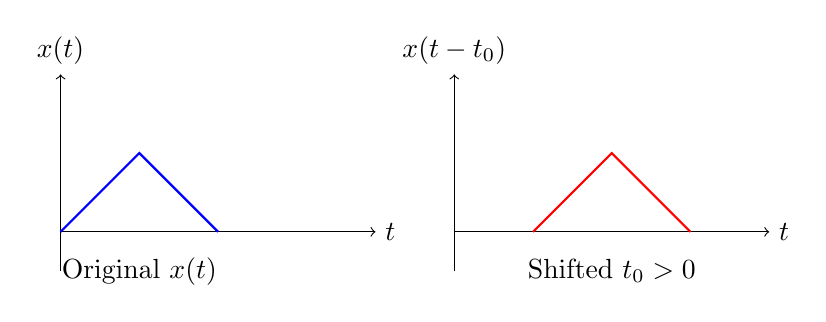
\begin{tikzpicture}
    % Original signal
    \draw[->] (0, 0) -- (4, 0) node[right] {$t$};
    \draw[->] (0, -0.5) -- (0, 2) node[above] {$x(t)$};
    \draw[thick, blue] (0, 0) -- (1, 1) -- (2, 0);
    \node at (1, -0.5) {Original $x(t)$};

    % Shifted signal
    \begin{scope}[shift={(5, 0)}]
        \draw[->] (0, 0) -- (4, 0) node[right] {$t$};
        \draw[->] (0, -0.5) -- (0, 2) node[above] {$x(t - t_0)$};
        \draw[thick, red] (1, 0) -- (2, 1) -- (3, 0);
        \node at (2, -0.5) {Shifted $t_0 > 0$};
    \end{scope}
\end{tikzpicture}

\subsection{Time Reversal}
A CT time reversal is given by $x(t) \rightarrow x(-t)$. A DT time reversal is given by $x[n] \rightarrow x[-n]$.

\begin{tikzpicture}
    % Original signal
    \draw[->] (-4, 0) -- (2, 0) node[right] {$t$};
    \draw[->] (0, -0.5) -- (0, 2) node[above] {$x(t)$};
    \draw[thick, blue] (-2, 0) -- (-1, 1) -- (0, 0);
    \node at (-1.5, -0.5) {Original $x(t)$};

    % Reversed signal
    \begin{scope}[shift={(5, 0)}]
        \draw[->] (-2, 0) -- (4, 0) node[right] {$t$};
        \draw[->] (0, -0.5) -- (0, 2) node[above] {$x(-t)$};
        \draw[thick, red] (0, 0) -- (1, 1) -- (2, 0);
        \node at (1.5, -0.5) {Reversed};
    \end{scope}
\end{tikzpicture}

\subsection{Time Scaling}
A CT time scaling is given by $x(t) \rightarrow x(\alpha t)$, where $\alpha > 0$ is the time scaling factor.
\marginnote{If $\alpha < 0$, that's viewed as a combination of reversal and scaling.}
\begin{itemize}
    \item $\alpha > 1$: shorter timescale, or sped up
    \item $\alpha < 1$: longer timescale, or slowed down
\end{itemize}
A DT time scaling is given by $x[n] \rightarrow x[\alpha n]$.

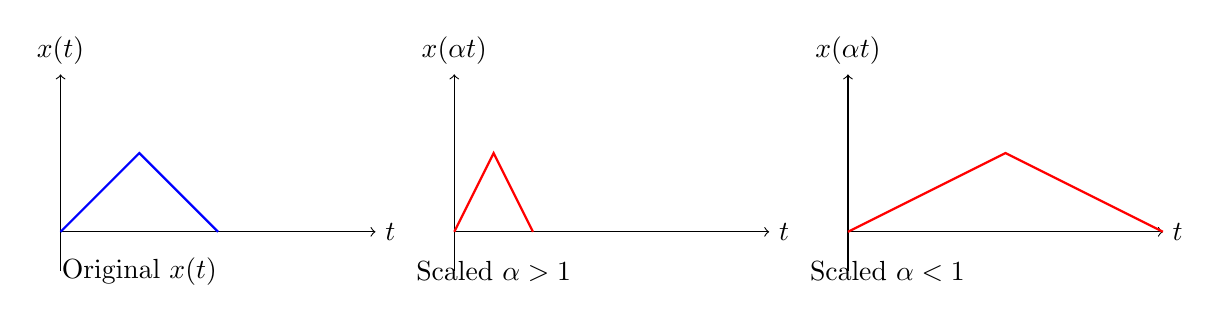
\begin{tikzpicture}
    % Original signal
    \draw[->] (0, 0) -- (4, 0) node[right] {$t$};
    \draw[->] (0, -0.5) -- (0, 2) node[above] {$x(t)$};
    \draw[thick, blue] (0, 0) -- (1, 1) -- (2, 0);
    \node at (1, -0.5) {Original $x(t)$};

    % Scaled signal
    \begin{scope}[shift={(5, 0)}]
        \draw[->] (0, 0) -- (4, 0) node[right] {$t$};
        \draw[->] (0, -0.5) -- (0, 2) node[above] {$x(\alpha t)$};
        \draw[thick, red] (0, 0) -- (0.5, 1) -- (1, 0);
        \node at (0.5, -0.5) {Scaled $\alpha > 1$};
    \end{scope}

    \begin{scope}[shift={(10, 0)}]
        \draw[->] (0, 0) -- (4, 0) node[right] {$t$};
        \draw[->] (0, -0.5) -- (0, 2) node[above] {$x(\alpha t)$};
        \draw[thick, red] (0, 0) -- (2, 1) -- (4, 0);
        \node at (0.5, -0.5) {Scaled $\alpha < 1$};
    \end{scope}
\end{tikzpicture}

